\documentclass[twocolumn, prd]{revtex4}
\usepackage{graphicx}
\begin{document}
\title{Putting  a Spark in Large Scale Astrophysical Computations}
\author{Meng et al.}
\begin{abstract}
We  argue for an early adoption of the rapidly maturing  Apache Spark {\url{http://spark.apache.org/}} engine based ecosystem for  big data computations in astrophysics, especially in the light of the LSST project.  Spark provides a unified framework for a large gamut of data analysis requirements in astrophysics. We motivate the adoption of Spark in astrophysics by describing several use cases. 
\end{abstract}
\maketitle
\section{Introduction}

\section{Map-reduce and Spark}
Map-reduce was first introduced at Google (Google BigTable) and since has emerged as an open source project with a vibrant community. Hadoop is a fault tolerant distributed file system designed for large scale data storage and data analysis. Map-Reduce is a divide and conquer algorithm that is used to analyze large datasets that are stored in Hadoop as Hadoop Distributed File System (HDFS). There are several Astrophysical computations where the computation can be broken down into small pieces with each piece being carried put independent of others. Map-Reduce paradigm can be extremely useful to parallelize these computations. One of the drawback of using Hadoop is the large latency of disk I/O. The map-reduce running on Hadoop cluster reads and writes many intermediate files to disk which makes the distributed computation slower to execute. Spark attempt to alleviate this problem by performing Map-reduce jobs in memory.  The  in-memory map reduce help in avoiding the disk I/O latency while still distributing the computations using Map-Reduce approach.
\section{Map-Reduce, hadoop vs. ground up MPI code}
There are two advantages of Hadoop- having a fault tolerant distributed file system, and distributing the computation. One might think if we don't need HDFS for our work and we can simply write a MPI based parallel program to distribute the computation, then what good is Hadoop plus the associated ecosystem. It is true one can write a MPI based parallelization, but one of the main advantage of  Map-Reduce and Hadoop ecosystem is to be able to parallelize the computation with minimum amount of effort from user. The only job of the user is to express the computation in Map and Reduce framework, and Hadoop takes care of the rest. As a result, one write relatively straight forward program with quick development time and still be able to massively parallelize the job.
\begin{figure}
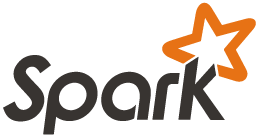
\includegraphics[width=0.4\linewidth]{spark-logo}
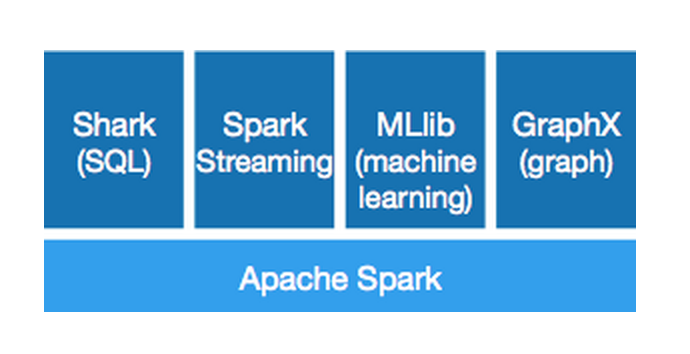
\includegraphics[width=\linewidth]{spark.png}
\caption{Spark powers a stack of high-level tools including Shark for SQL, MLlib for machine learning, GraphX, and Spark Streaming. These frameworks  cab be seamlessly combined in the same application.}
\end{figure}



\section{Types of Astrophysical Computations}
In the context of big data, there are three major types of Astrophysical computations: (a) \smallcaps{Query and aggregation}: frequent and fast query for astrophysical object over extensive databases, and summary statistics thereof; 
(b) \smallcaps{real time analysis:}  analysis of data as it streams from the telescope
(transients, supernovae, moving objects); (c) \smallcaps{analysis of archival data at scale:} classification, Fourier analysis, 
map-making, filtering, curve fitting, parameter estimation etc. on archival data. The standard in the astrophysical community has been applying different technologies for different problems: separate databases for queries, dedicated software stack for streaming analysis, and a slew of languages and platforms for archival data analysis.  This leads to frequent context switching for practitioners in the field, and makes it difficult to pursue projects that require live feedback between streaming analysis, querying and comparisons with archival data.  

\section{Where Spark Fits In}
Spark runs on top of  HDFS and enables querying databases via the Catalyst/Shark/BlinkDB SQL interface. The Spark Streaming tool enables real time analysis on streaming data (transients, supernovae, moving objects). Distributed machine learning  on archival  data sets (object detection, classification, photometric redshifts, supernova light curve fitting, etc.) can be performed using  MLLib,  a machine learning library built on top of Spark. Powerful statistical data exploration at scale can be performed with SparkR - a package for the R statistical language that enables R-users to leverage Spark functionality interactively from within the R shell. Relational (graph structured) data analysis can be performed using GraphX tool built on top of Spark.  Another great advantage of Spark is its Python API - pyspark -- that lets the end user develop applications in Python  -- a language that has already become extremely popular in  the astrophysics community. 



\section{Use Cases} 
\subsection{Finding Halos in Simulations and Halo Profile Calculation}
Halos are found in N-body simulations typically using friends-of-friends or spherical overdensity algorithm. The simulation volume can be divided into several small chunks (with buffer regions) on which the clustering algorithm can be run. The clustering algorithm (FOF or SO) itself can be broken into Map and Reduce steps and distributed across large number of compute nodes. 

Once the halos are found in the simulation, several halo specific statistics can be trivially Map-Reduced. E.g., concentration-mass calculation where each cluster is individually fitted using NFW or other profile and concentration of each clusters are then averaged over mass and redshift. 
\begin{enumerate}
\item Streaming/Real time analysis
	\subitem SNe
	\subitem  Near Earth Objects, GRBs, high velocity objects
\item Archival Data Analysis 
	\subitem  Objects detection 
	\subitem Correlation 
	\subitem Classification 
	\subitem  Photo-z 
	\subitem Light curve fitting 
\item Graph based algorithms 
\subitem Halo formation history, FoF - GraphX 
\subitem membership info (galaxies in a cluster etc.)
\item Simulation Data Analysis
\subitem Clustering algo? FoF/K-means++
\subitem Queries and relational analysis
\item Map making (CMB) SGD 
\item Dimensionality reduction
\end{enumerate}

\subsection{Finding Clusters from Survey data}
Similar to finding halos in the simulations, one can also find clusters of galaxies in observed data.



%%\section{Future Directions}
\end{document}